\documentclass[12pt]{article}

\usepackage[margin=1in]{geometry}
\usepackage{amsmath,amsthm,amssymb}
\usepackage{mathtools}
\usepackage{mathrsfs}
\usepackage{enumitem}
\usepackage{physics}
\usepackage{empheq}
\usepackage{undertilde}
\usepackage{float}
\usepackage{graphicx}
\graphicspath{ {./images/} }

\usepackage{tikz}
\usetikzlibrary{calc,decorations.markings,patterns}

\newcommand{\magsq}[1]{\big|#1\big|^2}
\newcommand{\avg}[1]{\left<#1\right>}
\newcommand{\fullint}{\int_{-\infty}^\infty}
\newcommand{\fullintd}[1]{\fullint\dd#1\:}
\newcommand{\cint}[2]{\int_{#1}^{#2}}
\newcommand{\cintd}[3]{\cint{#1}{#2}\dd#3\:}

\begin{document}

\title{Problem Set \#3}
\author{Phys 614}
\date{Due: 10:30 Noon, Thursday, May 16, 2023}
\maketitle

\section*{Problem 1}
The Sun is a sphere of radius $6.96 \times 10^5$ km with a surface temperature of 6000K. The Earth is $1.496 \times 10^8$ km from the Sun. Assuming that
\begin{enumerate}
    \item both the Earth's surface and the Sun's radiate as black bodies;
    \item there is no heat exchange between different points on the Earth's surface, 
    \item that each point on the Earth's surface equilibriates at a temperature that remains constant all day, and is such that it radiates exactly as much heat in the course of a day as it absorbes from the sun during the day, and
    \item The Earth is a perfect sphere;
\end{enumerate}
calculate the temperature $T(L)$ on the earth's surface at lattitude $L$ on March 21, the day that the Earth's axis is normal to the plane of the earth's orbit. Evaluate your answer for Eugene ($L=44^\circ$) and your home town. How well does the answer agree with your experience? \\
Note: lattitude is define as illustrated in Fig. 1.
\begin{figure}[H]
    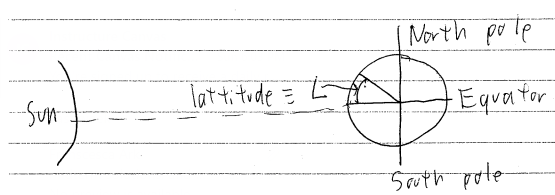
\includegraphics{Problem1}
    \centering
    \caption{The definition of lattitude.}
\end{figure}


\section*{Problem 2}
Hawking has argued that ``black holes ain't black'', rather, that they radiate due to the black holes' ``swallowing up'' one member of virtural particle-antiparticle pairs created near the schwarzschild radius, leaving the other to escape to infinity (see the discussion in Hawking's otherwise worthless ``A Brief History of Time''). The radiation thus emmitted has a black body spectrum (what else, for a black hole?). Assuming that the peak in this black body spectrum occurs at a wavelength comparable ot the schwarzschild radius $r_s$ of the black hole (defined as the radius at which the classical escape velocity equals the speed of light), calculate:
\begin{enumerate}[label=(\alph*)]
    \item The ``temperature'' of the black hole, as a function of its mass $M$.
    \item The total rate at which it emmits energy, assuming that the surface from which the emmision is occuring is a sphere of radius $r_s$. Express your answer solely in terms of $\hbar, M,$ the gravitational constant $G, $ and the speed of light $c$.
    \item Assuming all this emmitted energy is created by removing mass from the black hole, using $E=mc^2$, calculate the lifetime of a black hole as a function of its mass $M$. How does your answer compare with Hawking's statement that a black hole with the mass of the sun ($2\times 10^{30}$ kg) ``would take about $10^{66}$ years to evaporate completely''.
\end{enumerate} 

\section*{Problem 3}
Suppose the Earth was completely covered with a ``greenhouse gas'' which reflected back to the ground any radiation at wavelengths longer than visible light (i.e. $\lambda > 7\times 10^-7$m). What temperature $T_s$ would the earth's surface have to be to radiate away all of the heat recieved form the sun, assuming the surface was of \underline{uniform} temperature and radiated as a black body? \\
Hint: calculate the integrated emmission from all frequencies $\omega > \omega_\text{min} \equiv \frac{2\pi c}{\lambda_\text{max}}$, \underline{assuming}, to simplify the integral, that $\hbar\omega_\text{min} \gg k_B T_s$. You may also assume that \textit{all} of the sun's radiation reaches the earth's surface.

\end{document}